\chapter{Dynamic Programming}



\section{Introduction}
The core philosophy of dp:
\begin{enumerate}
\item The definition of \textbf{states} 
\item The definition of the \textbf{transition functions} among states 
\end{enumerate} 

The so called concept dp as memoization of recursion does not grasp the core philosophy of dp. 

The formula in the following section are unimportant. Instead, what is important is the definition of dp array and transition function derivation.
\subsection{Common practice}
\runinhead{Dummy.} Use dummies to avoid using if-else conditional branch.
\begin{enumerate}
\item Use $n+1$ dp arrays to reserve space for dummies. 
\item Iteration range is $[1, n+1)$.
\item $n+k$ for k dummies  
\end{enumerate}
\runinhead{State definition.} Two general sets of state definitions - the state 
\begin{enumerate}
\item ends \textit{at} index $i$
\item ends \textit{before} index $i$
\item ends \textit{at} or \textit{before} index $i$
\end{enumerate}

\runinhead{Space optimization.} To avoid MLE, we need to carry out space optimization. Let $o$ be other subscripts, $f$ be the transition function. 

Firstly,
$$
F_{i, o} = f\big(F_{i-1, o'}\big)
$$

should be reduced to 
$$
F_{o} = f\big(F_{o'}\big)
$$

Secondly,
$$
F_{i, o} = f\big(F_{i-1, o'}, F_{i-2. o'}\big)
$$

should be reduced to 
$$
F_{i, o} = f\big(F_{(i-1)\%2, o'}, F_{(i-2)\%2. o'}\big)
$$

More generally, we can be $(i-b)\%a$ to reduce the space down to $a$.

Notice:
\begin{enumerate}
\item Must iterate $o$ \textbf{backward} to un-updated value. 
\end{enumerate}



\section{Sequence}\label{dpSequence}
\runinhead{Longest common subsequence.} Let $F_{i, j}$ be the LCS at string $a[:i]$ and $b[:j]$. We have two situations: $a[i]==b[j]$ or not.
\begin{eqnarray*}
F_{i. j} = \left\{ \begin{array}{rl}
  F_{i-1, j-1}+1 &\mbox{// if $a[i]==b[j]$} \\
  \max\Big(F_{i-1, j},&\mbox{// otherwise} \\
  F_{i,j-1}\Big)
       \end{array} \right.
\end{eqnarray*}
\\
\runinhead{Longest common substring.} Let $F_{i, j}$ be the LCS at string $a[:i]$ and
$b[:j]$. We have two situations: $a[i]==b[j]$ or not.
\begin{eqnarray*}
F_{i. j} = \left\{ \begin{array}{rl}
  F_{i-1, j-1}+1 &\mbox{// if $a[i]==b[j]$} \\
  0 &\mbox{// otherwise}
       \end{array} \right.
\end{eqnarray*}

Because it is not necessary that $F_{i,j}\geq F_{i',j'}, \forall i,j\cdot i>i', j>j'$, the $gmax=max\big(\{{F_{i,j}\}\big)$.
\\
\runinhead{Maximum subarray sum.} Find the maximum subarray sum of $A$. 

Let $F_i$  be the maximum subarray sum ending at $A_{i}$
$$
F_i = \max(F_{i-1}+A_{i}, 0)
$$

Then the global $maxa$ is:
$$
maxa = \max(F_i\cdot \forall i)
$$


\runinhead{Maximum sum of non-adjacent cells.} Get the maximum sum of non-adjacent
cells of an array $A$.

Let $F_i$ be the maximum sum of non-adjacent cells for $A[:i]$. You have tow options:
choose $A_{i-1}$ or not.
\begin{align*}
F_{i} = \max\big(F_{i-1}, F_{i-2}+A_{i-1}\big)
\end{align*}
\runinhead{Edit distance} Find the minimum number of steps required to convert words $A$ to $B$ using inserting, deleting, replacing. 

Let $F_{i, j}$ be the minimum number
of steps required to convert $A[:i]$ to $B[:j]$.
\begin{eqnarray*}
F_{i, j} = \left\{ \begin{array}{rl}
  F_{i-1, j-1} &\mbox{// if $a[i]==b[j]$} \\
  \min\Big(F_{i, j-1}+1, &\mbox{// otherwise, insert}\\
  F_{i-1, j}+1, &\mbox{// delete}\\
  F_{i-1, j-1}+1\Big) &\mbox{// replace}\\
       \end{array} \right.
\end{eqnarray*}

\runinhead{Maximal square.} Find the largest rectangle in the matrix:
\begin{lstlisting}
1 0 1 0 0
1 0 1 1 1
1 1 1 1 1
1 0 0 1 0
\end{lstlisting}
Let $F_{i, j}$ represents the max square's length ended at $mat_{i, j}$ (lower right corner).
\begin{eqnarray*}
F_{i, j} = \left\{ \begin{array}{rl}
  \min\big(F_{i-1, j-1}, F_{i-1, j}, F_{i, j-1}\big)+1 &\mbox{// if $mat_{i, j}==1$} \\
  0 &\mbox{// otherwise}
       \end{array} \right.
\end{eqnarray*}

\runinhead{Maximal product subarray.} Find the subarray within an array $A$ which has the largest product. 
\begin{itemize}
\item Let $small_i$ be the smallest product end with $A_i$. 
\item Let $large_i$ be the largest product end with $A_i$.
\item The states can be negative. 
\end{itemize}
\begin{eqnarray*}
&& small_i = \min\big( A_i,\ small_{i-1}\cdot A_i,\ large_{i-1}\cdot A_i \big)
\nonumber \\
&& large_i = \max\big( A_i,\ small_{i-1}\cdot A_i,\ large_{i-1}\cdot A_i \big)
\end{eqnarray*}

It can be optimized to use space $O(1)$. 

\runinhead{Trapping Rain Water}
Given n non-negative integers representing an elevation map where the width of each
bar is 1, compute how much water it is able to trap after raining.
\begin{figure}[]
    \centerline{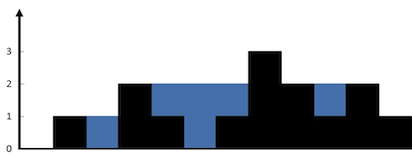
\includegraphics[height = 1in]{rainwatertrap}}
    \caption{Trapping Rain Water}
  \label{fig:rainwatertrap}
\end{figure}

Let $maxL_i$ be the $\max(A[:i])$; let $maxR_i$ be the $\max(A[i:n])$. The dp of obtaining max is trivial. 

The the total volume $vol$:
$$
vol = \sum_i(\max\big(0,\min(maxL_i, maxR_{i+1})-A[i]\big))
$$



\section{String}
\runinhead{Word break.} Given a string $s$ and a dictionary of words $dict$, determine if $s$ can be segmented into a space-separated sequence of $dict$ words.

Let $F_i$ be whether \pyinline{s[:i]} can be segmented. 
\begin{eqnarray*}
F_{i} = \left\{ \begin{array}{rl}
  F_{i-len(w)} &\mbox{// if $\exists w\in dict$, \pyinline{s[i-len(w):i]==w}}
\\
  false &\mbox{// otherwise}
       \end{array} \right.
\end{eqnarray*}
Return all such possible sentences. In original case, we use a bool array to record whether a dp could be segmented. Now we should use a vector for every dp to record how to construct that dp from another dp.

Let $F_i$ be all possible segmented words ends at \pyinline{s[i-1]}. $F_i$ is a list. 
\begin{eqnarray*}
F_{i} = \left\{ \begin{array}{rl}
  F_{i}+[w] &\mbox{// $\forall w\in dict\cdot$} \\
  & \mbox{ if \pyinline{s[i-len(w):i]==w} $\wedge\ \exists
F_{i-len(w)$ } \\
  F_{i}} &\mbox{// otherwise}
       \end{array} \right.
\end{eqnarray*}

Reconstruct the sentence from $F_i$. It is like building path for the tree. Using backtracking: 
\begin{python}
def build(self, dp, i, cur, ret):
    if cur_index == 0:
        ret.append(" ".join(list(cur)))
        return

    # backtracking
    for word in dp[i]:
        cur.appendleft(word)
        self.build(dp, i-len(word), cur, ret)
        cur.popleft()

\end{python}

\runinhead{Is palindrome.} Given a string $s$, use an array to determine whether $s[i:j]$.

Let $P_{i,j}$  indicates whether $s[i:j]$ is palindrome. We have one condition - whether the head and the end letter are equal: 
\begin{eqnarray*}
P_{i. j} = P_{i-1, j+1}\ \wedge\ s[i] = s[j-1]
\end{eqnarray*}

\runinhead{Minimum palindrome cut.} Given a string s, partition s such that every substring of the partition is a palindrome. Return the minimum cuts needed for a palindrome partitioning of s.

Let $C_i$ be the min cut for $s[:i]$. We have 1 more cut from previous state to make $S[:i]$ palindrome. 
\begin{eqnarray*}
C_{i} = \left\{ \begin{array}{rl}
  \min\big(C[k]+1 \cdot \forall k<i \big) &\mbox{// if $s[k:i]$ is palindrome}
\\
  0 &\mbox{// otherwise}
       \end{array} \right.
\end{eqnarray*}
\begin{python}
def minCut(self, s):
  n = len(s)

  P = [[False for _ in xrange(n+1)] for _ in xrange(n+1)]
  for i in xrange(n+1):  # len 0
    P[i][i] = True
  for i in xrange(n):  # len 1
    P[i][i+1] = True

  for i in xrange(n, -1, -1):  # len 2 and above
    for j in xrange(i+2, n+1):
      P[i][j] = P[i+1][j-1] and s[i] == s[j-1]

  C = [i for i in xrange(n+1)]  # max is all cut
  for i in xrange(n+1):
    if P[0][i]:
      C[i] = 0
    else:
      C[i] = min(
          C[j] + 1
          for j in xrange(i)
          if P[j][i]
      )

  return C[n]
\end{python}
\section{Backpack}
Given $n$ items with weight $w_i$ and value $v_i$, an integer $C$ denotes the size of a backpack. What is the max value you can fill this backpack?

Let $F_{i, c}$ be the max value we can carry for index $0..i$ with capacity $c$. We have 2 choices: take the $i$-th item or not.
\begin{eqnarray*}
F_{i, c}= \max\big(&&F_{i-1, c}, \\
&&F_{i-1, c-w_i}+v_i\big)
\end{eqnarray*}
Advanced backpack problem\footnote{\href{http://github.com/tianyicui/pack}{Nine Lectures in Backpack Problem}.}. 

\section{Local and Global Extremes}
\subsection{Long and short stocks}
The following formula derives from the question: Best Time to Buy and Sell Stock IV. Say you have an array for which the $i$-th element is the price of a given stock on day $i$. Design an algorithm to find the maximum profit. You may complete at most $k$ transactions. 

Let $local_{i, j}$ be the max profit with $j$ transactions with last transactions \textbf{ended at} day $i$. Let $global_{i, j}$ be the max profit with transactions \textbf{ended at} or \textbf{before} day $i$ with $j$ transactions. 

To derive transition function for $local$, for any given day $i$, you have two options: 1) transact in one day; 2) hold the stock one more day than previous and then transact. The latter option is equivalent to revert yesterday's transaction and instead transact today. 

To derive transition function for $global$, for any given day $i$, you have two options: 1) transact today; 2) don't transact today. 
\begin{eqnarray*}
&& local_{i,j} = \max\Big(global_{i-1.j-1}+\Delta, local_{i-1,j}+\Delta\Big) \nonumber \\
&& global_{i,j} = \max\Big(local_{i, j}, global_{i-1,j}\Big)
\end{eqnarray*}
, where $\Delta$ is the price change (i.e. profit) at day $i$.\\
Notice:
\begin{enumerate}
\item Consider opportunity costs and reverting transaction.
\item The global min is not $glocal[-1]$ but $\max\big(\{global[i]\}\big)$.
\item You must sell the stock before you buy again (i.e. you can not have higher than 1 in stock position). 
\end{enumerate}

\runinhead{Space optimization.}
\begin{eqnarray*}
&& local_{j} = \max\Big(global_{j-1} + \Delta, local_{j}+\Delta\Big)
\nonumber \\
&& global_{j} = \max\Big(local_{j}, global_{j}\Big)
\end{eqnarray*}

Notice,
\begin{enumerate}
\item Must iterate $j$ \textbf{backward}; otherwise we will use the updated value. 
\end{enumerate}

\runinhead{Alternative definitions.}
Other possible definitions: let $global_{i, j}$ be the max profit
with transactions ended at or before day $i$ with \textbf{up to} $j$ transactions. Then, 
\begin{eqnarray*}
&& local_{i,j} = \max\Big(global_{i-1.j-1} + \max(0, \Delta), local_{i-1,j}+\Delta\Big)
\nonumber \\
&& global_{i,j} = \max\Big(local_{i, j}, global_{i-1,j}\Big)
\end{eqnarray*}
and $global[-1]$ is the global max. 

The complexity of the alternative definitions is the same as the original definitions. The bottom line is that different definitions of states result in different transition functions.

\section{Game theory - multi players}
Assumption: the opponent take the optimal strategy for herself. 

\subsection{Coin game}
\runinhead{Same side} There are $n$ coins with different value in a line. Two players take turns to take 1 or 2 coins from left side. The player who take the coins with the most value wins.

let $F_i^p$ represents maximum values he can get for index $i..last$, for the person p. There are 2 choices: take the $i$-th coin or take the $i$-th and $(i+1)$-th coin.
\begin{eqnarray*}
F_i^p = \max\big(&A_i&+S[i+1:]-F_{i+1}^{p'},  \\
&A_i&+A_{i+1}+S[i+2:]-F_{i+2}^{p'}\big)
\end{eqnarray*}
The above equation can be further optimized by merging the sum $S$.

\runinhead{Dual sides}There are n coins in a line. Two players take turns to take a coin from one of the ends of the line until there are no more coins left. The player with the larger amount of money wins.

let $F_{i, j}^p$ represents maximum values he can get for index $i..j$, for
the person p. There are 2 choices: take the $i$-th coin or take the $j$-th coin.
\begin{eqnarray*}
F_{i,j}^p = \max\big(&A_i&+S[i+1:j]-F_{i+1,j}^{p'},  \\
&A_j&+S[i:j-1]-F_{i,j-1}^{p'}\big)
\end{eqnarray*}
